\documentclass[12pt,a4paper]{article}

%---packages----
\usepackage{setspace}
\usepackage{hyperref,enumerate,float,amsfonts,amssymb,amsmath,graphics,graphicx,mathtools}
\usepackage[margin=1.5 cm]{geometry}
\usepackage[T1]{fontenc}
\usepackage{bigfoot} % to allow verbatim in footnote
\usepackage[numbered]{matlab-prettifier}
\usepackage{graphicx}
\usepackage{listings}
\usepackage{xcolor}
\usepackage{color}
\usepackage{piton}
\usepackage{python}

%Adding References 
\usepackage[backend=bibtex,style=numeric]{biblatex} 
\addbibresource{references.bib}
\usepackage{hyperref,enumerate,float,amsfonts,amssymb,amsmath,graphics,graphicx,mathtools}
\usepackage[margin=1.5 cm]{geometry}
%\usepackage[hidelinks]{hyperref}



%----define colors----
\definecolor{codegreen}{rgb}{0,0.6,0}
\definecolor{codegray}{rgb}{0.5,0.5,0.5}
\definecolor{codepurple}{rgb}{0.58,0,0.82}
\definecolor{backcolour}{rgb}{0.95,0.95,0.92}


\setlength{\parindent}{0pt}

\lstdefinestyle{mystyle}{
    backgroundcolor=\color{backcolour},   
    commentstyle=\color{codegreen},
    keywordstyle=\color{magenta},
    numberstyle=\tiny\color{codegray},
    stringstyle=\color{codepurple},
    basicstyle=\ttfamily\footnotesize,
    breakatwhitespace=false,         
    breaklines=true,                 
    captionpos=b,                    
    keepspaces=true,                 
    numbers=left,                    
    numbersep=5pt,                  
    showspaces=false,                
    showstringspaces=false,
    showtabs=false,                  
    tabsize=2
}

\lstset{style=mystyle}


\lstdefinestyle{mystyle}{
numbers = none,
basicstyle=\ttfamily
}

\let\ph\mlplaceholder % shorter macro
\lstMakeShortInline"

\lstset{
 style              = Matlab-editor,
  basicstyle         = \mlttfamily,
%  escapechar         = ",
  mlshowsectionrules = true,
}

\onehalfspacing

%-----------------------------------------------------------------
%------------------
%      document begin
%------------------
%-----------------------------------------------------------------
\begin{document}

\begin{titlepage}


\newcommand{\HRule}{\rule{\linewidth}{0.5mm}} % Defines a new command for the horizontal lines, change thickness here

\center % Center everything on the page

%----------------------------------------------------------------------------------------
%	LOGO SECTION
%----------------------------------------------------------------------------------------



%----------------------------------------------------------------------------------------
%	HEADING SECTIONS
%----------------------------------------------------------------------------------------



%----------------------------------------------------------------------------------------
%	TITLE SECTION
%----------------------------------------------------------------------------------------

\makeatletter

\HRule \\[0.4cm] %Make horizontal line with space after 0.4cm

 % Title of your document
\huge{\bfseries \@g  Main\_title}

\HRule \\[1.5cm] %Make horizontal line with space before 1.5cm


%-----------------------------------------------------------------
%------------------
%      VERTICAL SPACE 
%------------------
%-----------------------------------------------------------------

\vfill % Fill the rest of the page with whitespace
\vspace*{\fill}
%----------------------------------------------------------------------------------------

\end{titlepage}

%----------------------------------------------------------------------------------------
%	starting sections of document
%----------------------------------------------------------------------------------------
\newpage
\section*{Preface}

%----------------------------------------------------------------------------------------
%	AUTHOR SECTION
%----------------------------------------------------------------------------------------
\begin{LARGE}
\begin{tabular}{l l}
Nada Atia Eid & ......... \\

\end{tabular} 
\end{LARGE}

\newpage
\section*{Acknowledgement}
\newpage
% Table of Contents
\tableofcontents
\newpage 

% List of Tables
\listoftables
\newpage 

% List of Figures
\listoffigures
\newpage 
\newpage
\section*{Abstract}


Driver fatigue and distraction pose significant risks to road safety, emphasizing the critical need for Driver Monitoring Systems (DMS). These systems are pivotal in detecting and mitigating driver impairment, thereby improving overall road safety standards. However, existing solutions often face challenges related to real-time responsiveness and accuracy, which are crucial for effectively preventing accidents caused by distracted or drowsy driving.

\vspace{\baselineskip}

In response to these urgent challenges, this project aims to develop an innovative driver monitoring system. The primary objective is to create a robust system capable of classifying driver states into four categories: focused, sleepy, distracted, and drowsy. The system achieves this classification using a combination of computer vision and machine learning techniques. Key features include eye closure detection, gaze tracking, yawn detection, and head pose estimation, all fed from an infrared camera to ensure functionality under various lighting conditions.

\vspace{\baselineskip}

This system harnesses the capabilities of the Texas Instruments TDA4VM System on Chip (SoC), renowned for its high-performance computing tailored for automotive applications. By leveraging the TDA4VM SoC's dual-core 64-bit Arm Cortex-A72 processors, DSPs, and deep-learning accelerators, the system delivers high-performance, real-time driver monitoring. All processing is conducted on the edge, directly on the TDA4VM SoC, eliminating the need for distributed processing on external devices such as laptops or cloud servers. This design ensures the system is ready for seamless integration into smart car systems, providing a self-contained, real-time monitoring solution.

\vspace{\baselineskip}

Experimental results demonstrate the system's ability to accurately detect and classify driver states with a final accuracy of \textcolor{red}{90\%} and a processing rate of \textcolor{red}{17} frames per second (FPS). The results indicate significant improvements in both detection accuracy and system responsiveness, confirming the efficacy of the TDA4VM SoC in automotive safety applications.

\vspace{\baselineskip}

Moreover, we provide a mobile application and \textcolor{red}{communication module} to fit various use cases. This addition will allow for remote monitoring and alerts, facilitating scenarios such as fleet management or caregiver notifications. The mobile app will enable users to view real-time driver status updates, receive alerts for potential fatigue or distraction events, and access historical data for analysis and reporting purposes.

\vspace{\baselineskip}

By combining advanced hardware capabilities with user-friendly mobile applications, this integrated solution not only aims to elevate safety standards within vehicles but also sets a precedent for future innovations in automotive safety technology.


\newpage
\section*{Introduction}


\newpage
\section{AI  System Solution}
The main application continuously analyzes the driver’s state, focusing on age and gender prediction, drowsiness detection, and distraction detection using artificial intelligence methods. The system captures and processes video data in real-time by utilizing infrared (IR) or RGB images.\\

Our approach simplifies the process by using a deep learning model for face detection and classical machine learning and image processing techniques for further analysis. After detecting faces, the system extracts facial landmarks. These landmarks are then used to estimate head pose, monitor eye and mouth aspect ratios, and track eye gaze direction to identify signs of drowsiness and distraction.\\

This method is computationally efficient, enabling real-time performance, and adaptable to different lighting conditions. 

\subsection{ Face Feature Extraction}

In driver monitoring systems, the extraction of facial features plays a critical role in ensuring accurate and reliable detection of driver states such as drowsiness and distraction. This process involves several key steps, each contributing to the system's overall effectiveness. The system's design is depicted in Fig. 1. The DMS employs a camera (imager) as the input image source, and the captured image is used for face detection followed by facial landmarks estimation. These extracted facial landmarks serve as crucial features for estimating head pose and identifying instances of closed eyes and yawning, indicative of drowsy driving.

\subsubsection{Face Detection Using YOLOv8n}

The first step in facial feature extraction involves detecting the driver's face using YOLOv8, or You Only Look Once version 8. YOLOv8 is a 1-stage detection algorithm, similar to the SSD detector, offering both satisfactory performance and fast processing speed, specifically the nano version implemented by Ultralytics. As shown in Fig. 2, the nano version is chosen for its efficient use of computational resources without compromising on detection accuracy, making it ideal for real-time applications in resource-constrained environments. \\

Trained on the comprehensive WIDERFACE dataset. The WIDERFACE dataset is a large and diverse collection of over 32,000 images with nearly 400,000 labeled faces, designed to cover a wide range of challenging real-world scenarios for robust face detection.\\

The model generates bounding boxes that precisely outline each detected face, defined by coordinates for the top-left corner and dimensions. These bounding boxes are accompanied by confidence scores, quantifying the model's certainty that the box contains a face. \\

PyTorch was selected for training YOLO over TensorFlow for deployment in C++ environments and its capability to load models directly into memory, resulting in faster inference times crucial for real-time applications. PyTorch's support for seamless deployment across GPUs, CPUs, and custom accelerators ensures scalability and performance optimization. Additionally, its superior support for multithreading enhances efficiency in handling concurrent tasks, making it suitable for high-throughput applications.\\

\subsubsection{ Facial Landmarks Extraction}

Facial landmark extraction has made significant strides in recent years, with deep learning techniques like Openface and Retinaface at the forefront. However, in our DMS, the high computational costs associated with face detection using deep learning present a challenge. To mitigate this, we have chosen Kazemi's fast facial landmark extraction algorithm, which has been integrated into the Digital Library (Dlib) library. Kazemi’s algorithm, based on random forests, provides an excellent balance of speed and performance, making it suitable for the DMS, which needs to function efficiently in an embedded environment rather than a desktop setup.\\

Dlib's first step is face detection, then applying facial landmark extraction built on Kazemi's algorithm's principles. Dlib includes two face detection methods:
\begin{enumerate}
    \item HOG + Linear SVM Face Detector: \\
    This method accessible via dlib.get\_frontal\_face\_detector(), is known for its accuracy and computational efficiency.
    \item Max-Margin (MMOD) CNN Face Detector: \\
    This method is highly accurate and robust, capable of detecting faces under varying viewing angles, lighting conditions, and occlusion.
\end{enumerate}

For our system, we replace the HOG + Linear SVM face detection method with the YOLOv8 face detection model. YOLOv8 provides more accurate and faster face detection, which is crucial for the real-time requirements of our DMS. By leveraging the precise bounding boxes generated by YOLOv8, we can then feed these into Dlib for accurate facial landmarks. This is crucial for analyzing the driver's state, and detailed explanations of their use will be provided in subsequent sections.\\

We use the shape\_predictor\_68\_face\_landmarks\_GTX.dat.bz2 model, a highly optimized and accurate facial landmark detector. This model is trained on the ibug 300-W dataset, a comprehensive benchmark dataset containing a variety of images with annotated facial landmarks. The GTX version of the model utilizes advanced training strategies to enhance performance and accuracy, including data augmentation, robust optimization techniques, and meticulous fine-tuning to ensure the model can accurately predict 68 key facial landmarks under diverse conditions.\\

The output of this stage is the key 68 landmarks, which are then fed into other algorithms for further analysis. This integration ensures that our DMS can reliably monitor the driver states.

\subsubsection{Age and Gender Estimation}

In the context of diver monitoring systems, estimating the age and gender of divers is crucial for several reasons:

\begin{enumerate}
    \item \textbf{Safety Protocols:} Different age groups and genders may have varying physiological responses to underwater conditions. Understanding these differences can help tailor safety protocols to ensure the well-being of all divers.
\item \textbf{Personalized Experiences: }Personalized recommendations and experiences can enhance a diver's overall satisfaction. For instance, training programs can be customized based on the age and gender of the divers.
\item \textbf{Statistical Analysis:} Collecting demographic data allows for detailed analysis of diving patterns and trends, aiding in the development of targeted marketing strategies and improvement of services.
\end{enumerate}

\textbf{Models Provided by Dlib and Cydral Technology}\\
The pre-trained models for age and gender estimation used in this system are provided by Dlib and are available for free under the Creative Commons Zero v1.0 Universal license by Cydral Technology. These models offer robust performance due to their training on large, private datasets and their sophisticated architectures.\\

\textbf{Gender Classifier: "dnn\_gender\_classifier\_v1.dat.bz2"}\\
This gender classifier model was trained on approximately 200,000 face images. The training followed the architecture and settings outlined in the paper "Minimalistic CNN-based ensemble model for gender prediction from face images." Key features include:
\begin{itemize}
    \item \textbf{CNN Ensemble Model:} The use of a minimalistic CNN ensemble approach helps improve classification accuracy by leveraging multiple CNNs.
\item \textbf{Private Dataset:} The extensive dataset ensures that the model generalizes well to diverse real-world scenarios.
\end{itemize}











\subsection{Eye Closure Detection}

In our previous discussions, we explored how to apply facial landmark detection to identify key regions of the face, such as the eyes, eyebrows, nose, ears, and mouth. This capability allows us to extract specific facial structures by referencing the indexes of particular face parts.

\begin{figure}[H]
    \centering
    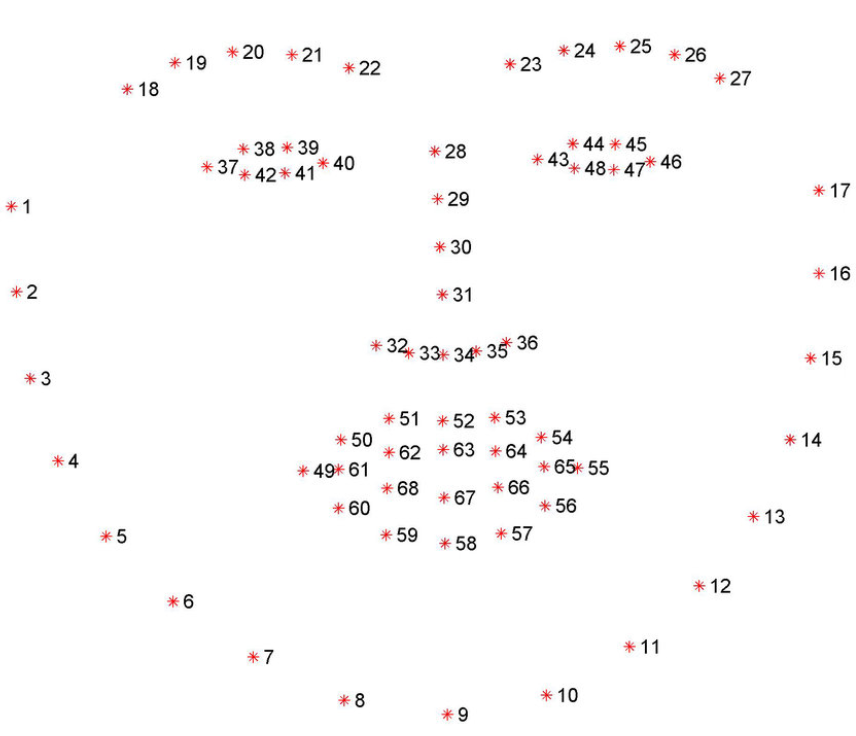
\includegraphics[width=0.7\textwidth]{Images/1_AI/68_face_landmarks.png}
    \caption{Applying facial landmarks to localize various regions of the face, including eyes, eyebrows, nose, mouth, and jawline.}
    \label{fig:68_face_landmarks}
\end{figure}

For the purpose of blink detection, we focus on two sets of facial structures: the eyes.

Each eye is represented by six (x, y)-coordinates, starting at the left corner of the eye (as if you were looking at the person) and moving clockwise around the rest of the region.

\begin{figure}[H]
    \centering
    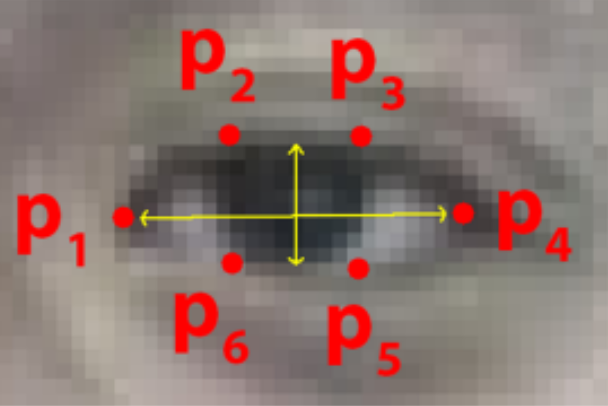
\includegraphics[width=0.5\textwidth]{Images/1_AI/6points_open_eye.png}
    \caption{The six facial landmarks associated with the eye.}
    \label{fig:6points_open_eye}
\end{figure}

Building on the work by Soukupová and Čech in their 2016 paper, *Real-Time Eye Blink Detection using Facial Landmarks*, we derive an equation reflecting this relationship, known as the eye aspect ratio (EAR):

\begin{equation}
\text{EAR} = \frac{\|p_2 - p_6\| + \|p_3 - p_5\|}{2 \|p_1 - p_4\|}
\end{equation}

where \( p_1, \ldots, p_6 \) are 2D facial landmark locations. The numerator calculates the distance between the vertical eye landmarks, while the denominator computes the distance between horizontal eye landmarks, with appropriate weighting since there is only one set of horizontal points but two sets of vertical points.

The eye aspect ratio remains approximately constant when the eye is open but rapidly decreases to zero when a blink occurs. This simple equation enables us to detect blinks by relying on the ratio of eye landmark distances, bypassing the need for complex image processing techniques.

Consider the following figures:

\begin{figure}[H]
    \centering
    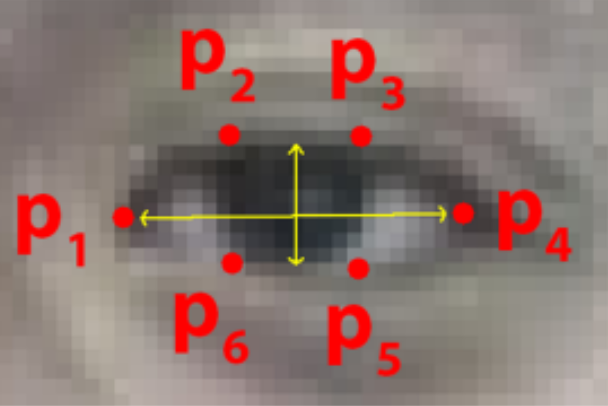
\includegraphics[width=0.8\textwidth]{Images/1_AI/6points_open_eye.png}
    \caption{Eye landmarks when the eye is open.}
    \label{fig:6points_open_eye}
\end{figure}

\begin{figure}[H]
    \centering
    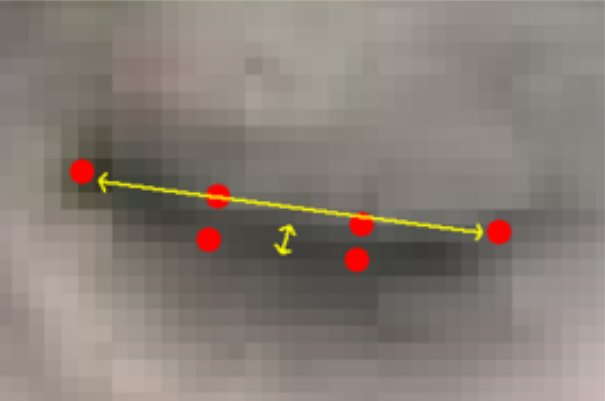
\includegraphics[width=0.8\textwidth]{Images/1_AI/6points_closed_eye.png}
    \caption{Eye landmarks when the eye is closed.}
    \label{fig:6points_closed_eye}
\end{figure}

\begin{figure}[H]
    \centering
    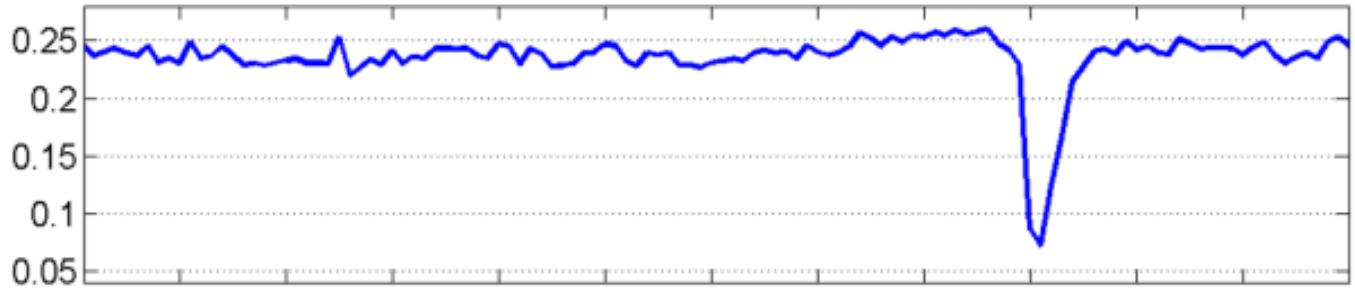
\includegraphics[width=0.8\textwidth]{Images/1_AI/ear_over_time.png}
    \caption{Plotting the eye aspect ratio over time. The dip in the eye aspect ratio indicates a blink.}
    \label{fig:ear_over_time}
\end{figure}

In Figure \ref{fig:Eye_landmarks_open}, the eye is fully open, and the eye aspect ratio is relatively large and constant. When the person blinks (Figure \ref{fig:Eye_landmarks_closed}), the eye aspect ratio drops significantly, approaching zero.

To determine whether the eye is open or closed based on the Eye Aspect Ratio (EAR), a threshold value is crucial. Typically, the eye is classified as closed when the EAR drops below a specified threshold, such as the commonly recommended value of around \textcolor{red}{0.25}. This value ensures accurate detection of blinks and prolonged eye closures, critical for evaluating driver alertness in driver monitoring systems. Adjusting the threshold to approximately \textcolor{red}{0.25} enhances performance under different lighting conditions and facial orientations.

Figure \ref{fig:ear_over_time} plots the eye aspect ratio over time for a video clip. As observed, the eye aspect ratio remains constant, then drops near zero, and rises again, indicating a blink.

\newpage

\subsection{Yawn Detection}

Yawn detection is another crucial indicator of driver fatigue. This detection algorithm analyzes the distance between the upper and lower lips using facial landmarks.

The algorithm calculates the mean positions of the upper and lower lips using the following steps:

\subsubsection*{1. Calculate the Mean Positions of the Outer Upper Lip Landmarks}

\[
\text{upper\_mean}_x = \frac{x_{u50} + x_{u51} + x_{u52} + x_{u61} + x_{u62} + x_{u63}}{6}
\]

\[
\text{upper\_mean}_y = \frac{y_{u50} + y_{u51} + y_{u52} + y_{u61} + y_{u62} + y_{u63}}{6}
\]

\subsubsection*{2. Calculate the Mean Positions of the Outer Lower Lip Landmarks}

\[
\text{lower\_mean}_x = \frac{x_{l56} + x_{l57} + x_{l58} + x_{l65} + x_{l66} + x_{l67}}{6}
\]

\[
\text{lower\_mean}_y = \frac{y_{l56} + y_{l57} + y_{l58} + y_{l65} + y_{l66} + y_{l67}}{6}
\]

\subsubsection*{3. Compute the Vertical Distance Between the Mean Positions}

\[
\text{distance} = \left| \text{upper\_mean}_y - \text{lower\_mean}_y \right|
\]

\begin{figure}[H]
    \centering
    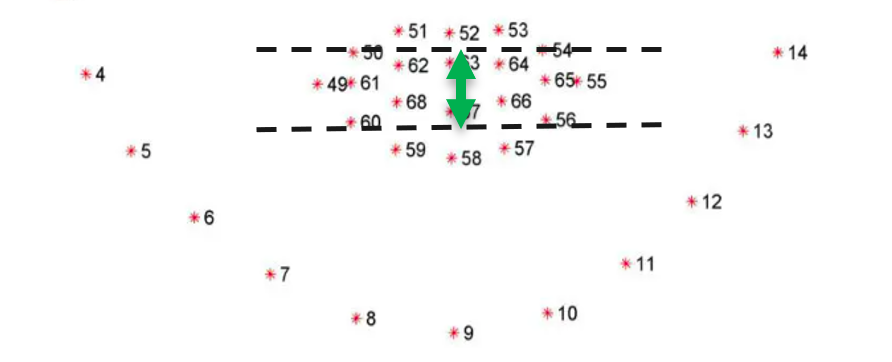
\includegraphics[width=0.7\textwidth]{Images/1_AI/yawn_distance.png}
    \caption{Facial landmarks for yawning detection.}
    \label{fig:yawn_distance}
\end{figure}

By measuring the distance between the upper and lower lip landmarks (Figure \ref{fig:yawn_distance}), the algorithm can determine if the mouth is open, which is a key indicator of yawning. A significant increase in this distance indicates a yawn, suggesting that the driver may be fatigued.

Yawning detection also relies on a threshold, often determined by the vertical distance between upper and lower lip landmarks. While specific thresholds can vary, values around \textcolor{red}{0.5 to 1.0} have been used experimentally. Adjusting this threshold helps in accurately identifying yawning events, crucial for assessing driver fatigue in monitoring systems, despite varying facial expressions and conditions.

By integrating these advanced detection methods, the driver monitoring system can effectively assess driver fatigue and drowsiness, contributing to improved road safety.

\newpage
\section{SIL}

\newpage
\section{Decision Layer}
\newpage
\section{Hardware Selection}
\subsection{Camera Selection for Driver Monitoring Systems (DMS)}

In embedded vision applications, particularly within Driver Monitoring Systems (DMS), the camera serves as the primary sensor, capturing essential visual data for analysis. The selection of an appropriate camera is crucial to ensure accurate monitoring of the driver's face, eyes, and upper body movements. This section outlines key criteria for camera selection to optimize the effectiveness of DMS.

\subsubsection{\textbf{Image Sensor} (CCD vs. CMOS)}


\begin{figure}[!h]
     \centering
     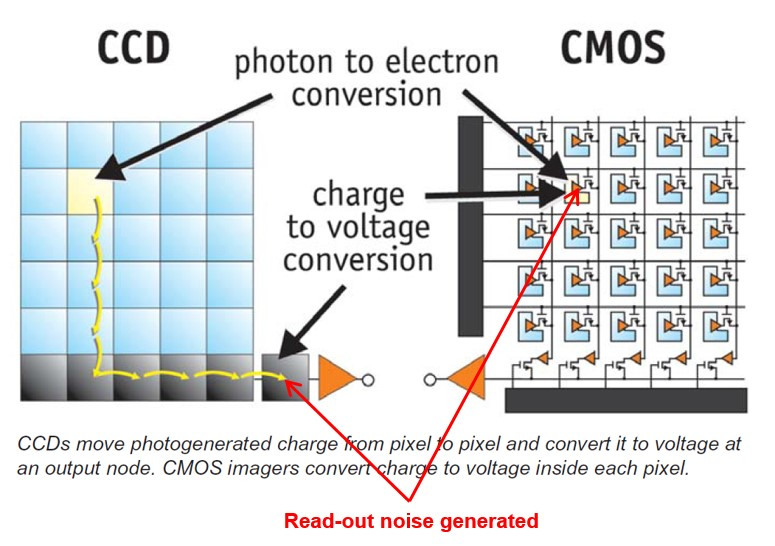
\includegraphics[scale =0.3]{Images/4.1_Camera_Selection/CCDVsCMOS.jpg}
     \caption{CCD vs. CMOS Operation}
     \label{fig:CCDVsCMOS}
\end{figure}

The debate between CCD (Charge-Coupled Device) and CMOS (Complementary Metal-Oxide-Semiconductor) sensors has shaped the evolution of digital cameras, particularly in still photography. As shown in Figure \ref{fig:CCDVsCMOS}, CCD sensors dominated early digital cameras for their superior image quality and specific applications.They operate on a charge-transfer mechanism with a serial process requiring mechanical shutters to prevent smear artifacts during readout. In contrast, CMOS sensors gained prominence with their parallel readout capability, enabling faster processing, lower power consumption, and integration with advanced functionalities like live-view and electronic shutters. Canon's introduction of the first full-frame CMOS sensor in 2002 marked a significant milestone, accompanied by sensor design and manufacturing advancements. Objectively, CCD sensors offer superior image quality with accurate color rendition and smooth tonal transitions but consume more power, generate heat, and have slower readout speeds. CMOS sensors, on the other hand, provide faster readout speeds, lower power consumption, and improved noise performance, particularly in low-light conditions, enhanced further by innovations like Backside Illumination (BSI). Subjectively, while CCD sensors excel in scenarios requiring precise color fidelity and minimal noise at base ISO, CMOS sensors are versatile, supporting high-speed continuous shooting, video recording, and real-time viewing, aligning well with evolving industry demands.

For DMS, CMOS technology is preferred due to its lower power consumption, superior noise performance, and compatibility with real-time video processing, making it ideal for capturing detailed driver behavior effectively.

\subsubsection{\textbf{Shutter Type} (Global Vs. Rolling)}
Exposure time is a period of the shutter from open to close. During the period, the light exposing on the chip’s photosensitive array and Photoelectric effect occurs. After that, photoelectric charges are produced. By the A/D transformation, the value of each pixel is displayed. Under a certain light intensity, the longer the shutter is open, the longer the exposure time, the brighter the image. Long exposure time can show the trajectory of slow moving objects on an image. Short exposure time can record things more accurately. 

In digital cameras, there is usually no mechanical shutter which determines the exposure time. Instead, an electronic shutter is used. This process involves resetting the pixel just before the exposure period starts to return it to its initial state. At the end of the exposure period, the pixel is read out to capture the signal generated by the incident light. Two types of electronic shutters can be used: global shutter and rolling shutter, which differ in their timing mechanisms.

\begin{figure}[!h]
     \centering
     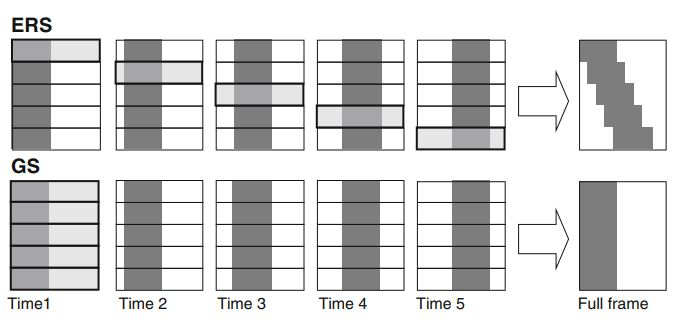
\includegraphics[scale =0.8]{Images/4.1_Camera_Selection/GlobalVsRolling.jpg}
     \caption{Difference of electronic rolling shutter (ERS) and global shutter (GS)}
     \label{fig:GlobalVsRolling}
\end{figure}


As shown in Figure \ref{fig:GlobalVsRolling}, in global shutter mode, each pixel in the sensor begins and ends the exposure simultaneously. This mode requires a significant amount of memory, as the entire image must be stored in memory after the exposure ends and can then be read out gradually. The manufacturing process for global shutter sensors is relatively complex, making them more expensive. However, the advantage of a global shutter is its ability to capture high-speed moving objects without distortion, making it suitable for a wide range of applications.

In rolling shutter mode, different lines of the sensor array are exposed at different times as the readout sweeps through the sensor, as shown in Figure \ref{fig:GlobalVsRolling}. The first line is exposed first, followed by a readout period, then the second line starts exposure, and so on. This sequential exposure means each line reads out before the next line begins. Each pixel in a rolling shutter sensor requires only two transistors to transport electrons, resulting in lower heat production and reduced noise. Compared to global shutter sensors, rolling shutter sensors have a simpler structure and lower cost. However, because each line is not exposed simultaneously, rolling shutters can produce distortion when capturing high-speed moving objects, as shown in figure \ref{fig:GlobalVsRolling2}.

\begin{figure}[!h]
     \centering
     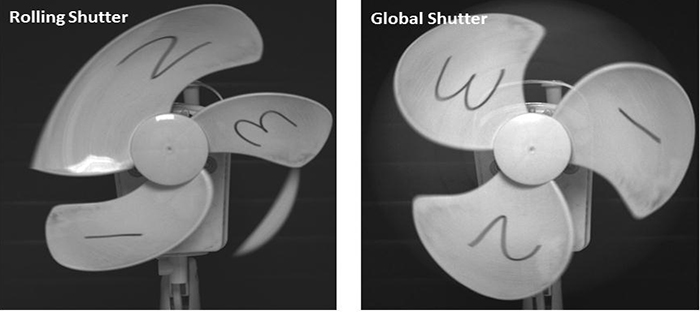
\includegraphics[scale =0.6]{Images/4.1_Camera_Selection/GlobalVsRolling2.jpg}
     \caption{Comparison of rolling and global shutter in high-speed imaging of moving objects}
     \label{fig:GlobalVsRolling2}
\end{figure}

For DMS applications, where accurately capturing the driver's movements and behaviors in real-time is crucial, the global shutter is the preferred choice.



\subsubsection{\textbf{Monochrome vs. Color Camera Modules}}

\textbf{Monochrome Camera Module} \\
Monochrome camera modules capture images exclusively in shades of gray. 

One significant advantage of monochrome cameras is their higher sensitivity to light compared to color cameras. This increased sensitivity is due to the absence of a color filter array, which allows more light to reach the sensor. Consequently, monochrome cameras can capture clearer and sharper images in low-light conditions.

Additionally, monochrome cameras offer higher resolution. Each pixel in a monochrome camera captures all incoming light, whereas each pixel in a color camera captures only one color. This results in monochrome cameras being able to capture more details and produce higher-quality images.

However, a notable limitation of monochrome cameras is their inability to capture color images. If color information is essential for application, a color camera is necessary. Furthermore, monochrome cameras are typically more expensive than color cameras.

\textbf{Color Camera Module} \\
Color camera modules capture images in full color with many types of color filter arrays.

An advantage of color cameras is their ability to capture images in full color, which is crucial for applications requiring color information. Additionally, color cameras are generally more affordable than monochrome cameras, making them popular for consumer applications like smartphones and digital cameras.

Another benefit of color cameras is their ability to capture images at a faster rate. The color filter array in these cameras allows them to capture all three primary colors (red, green, and blue) simultaneously, enabling faster image capture.

However, color cameras have a lower sensitivity to light compared to monochrome cameras. The color filter array reduces the amount of light reaching the sensor, which can result in less sharp and detailed images in low-light conditions.

For applications like DMS, requiring high sensitivity and detailed resolution, especially in low-light conditions, monochrome cameras are preferable.

\subsubsection{\textbf{Protocol and Interface}}

When designing DMS system, selecting the optimal interface for transmitting visual information is critical to its overall performance. This interface serves as the physical connection layer that links the camera to the processing platform, facilitating image transmission and subsequent processing. Key considerations include throughput capabilities and transmission distance.

In response to increasing demands for high-speed connectivity, the market offers a range of flexible and robust interfaces. Among the most widely adopted are MIPI CSI-2, GMSL, and USB interfaces, each tailored to meet specific industry needs

\textbf{MIPI CSI-2}\\ 
MIPI CSI-2, or Mobile Industry Processor Interface Camera Serial Interface Type-2, is a high-speed serial interface primarily developed for transmitting image and video data from mobile camera modules to embedded processors. Originally designed for mobile devices, MIPI CSI-2 has found widespread adoption in mobile phones, tablets, and handheld embedded systems due to its versatility and performance capabilities.

The interface supports a peak bandwidth of 6 Gbps, with a practical bandwidth typically around 5 Gbps. It utilizes four image data lanes, each capable of transmitting up to 1.5 Gbps, surpassing the speed of USB 3.0. MIPI CSI-2 is renowned for its efficiency and reliability, capable of handling video resolutions ranging from 1080p to 8K and beyond. It also minimizes CPU resource consumption, leveraging the capabilities of multi-core processors.

MIPI CSI-2 is designed with low power consumption in mind, making it well-suited for battery-powered embedded devices. Its scalability, enabled by multiple data lanes, allows for flexible adjustment of data transfer rates based on application requirements. The interface employs a differential signaling scheme, enhancing noise immunity and ensuring high reliability in data transmission.

However, MIPI CSI-2 has limitations, including a maximum supported cable length of 30 cm, which restricts its use over longer distances. Additionally, implementing MIPI CSI-2 requires specialized components, potentially increasing the cost of the embedded system.

\textbf{USB} \\
USB (Universal Serial Bus) is a widely adopted data transfer protocol in computing devices and embedded systems. In embedded vision systems, USB 2.0 and 3.0 protocols serve as common interfaces for transferring image and video data from camera sensors to host processors.

USB 2.0 supports a maximum data transfer rate of 480 Mbps, while USB 3.0 significantly increases this bandwidth to 5 Gbps. These interfaces are extensively utilized in embedded vision applications such as surveillance systems, industrial inspection, and machine vision, particularly favored for their low-cost and low-power attributes.

The plug-and-play capability is a notable advantage of USB camera interfaces, simplifying integration and reducing development costs. USB 3.0, with its higher bandwidth of up to 360 MB/s, aligns well with the USB3 Vision Standard in embedded vision systems, facilitating seamless device replacement and enhancing flexibility.

However, USB interfaces have limitations. Both USB 2.0 and 3.0 support a maximum cable length of 5 meters, which can restrict deployment options. Additionally, these interfaces lack dedicated video streaming capabilities, potentially causing delays or loss of image data during transmission.\\

\textbf{GMSL} \\
Gigabit Multimedia Serial Link (GMSL) is a high-speed serial link protocol designed primarily for transmitting image and video data in embedded vision systems, particularly in automotive applications. GMSL enables the transmission of high-speed video, bidirectional control data, and power over a single coaxial cable, supporting distances of up to 15 meters with low latency and high frame rates.

GMSL utilizes differential pair transmission for enhanced noise immunity and data integrity. Its unique encoding scheme reduces electromagnetic interference (EMI), allowing for longer cable lengths and higher data rates compared to traditional serial link interfaces.

Commonly used in ADAS (advanced driver assistance systems), autonomous vehicles, and quality control systems, GMSL is favored for its high bandwidth, reliability, and suitability for long-distance transmission.

However, GMSL interfaces tend to be more expensive than alternatives like USB due to the specialized hardware and software required. Additionally, the protocol's complexity may pose challenges for users unfamiliar with its implementation.\\

In our project, we have chosen MIPI CSI-2 as the interface for transmitting visual information due to its compelling advantages in affordability and reliability. MIPI CSI-2 offers high-speed data transfer capabilities, making it well-suited for handling high-resolution video streams efficiently. Its low power consumption is crucial for our battery-powered application, ensuring extended operational lifetimes without compromising performance.

While MIPI CSI-2 excels in these areas, it's worth noting its limitations compared to USB and GMSL interfaces. Specifically, MIPI CSI-2 supports shorter cable distances compared to USB's 5-meter limit and GMSL's ability to extend up to 15 meters. This constraint may impact flexibility in our system setup but is outweighed by MIPI CSI-2's overall suitability for our application's needs.



\newpage
\section{App Deployment}
\subsection{Camera integration}
In our DMS, we integrate the 8-megapixel IMX219-160IR Camera from Waveshare. 
The camera features a CMOS sensor with a resolution of 3280 x 2464 pixels and a 1/4-inch sensor size. With an aperture of 2.35 and a focal length of 3.15mm, it offers a wide diagonal field of view (FOV) of 160 degrees, crucial for capturing a broad area within the vehicle cabin. The lens, measuring 6.5mm x 6.5mm, minimizes distortion to less than 14.3\%, ensuring accurate image representation for effective driver monitoring applications.

\subsubsection{\textbf{Camera interface}}
Data and clock signals are transmitted using CSI-2 interface utilizing 2Lanes Outputs of data and clock come from CSI-2 output pins (DMO1P/DMO1N, DMO2P/DMO2N, DCKP/DCKN). A pair of DMO1P/DMO1N is called Lane1 data and a pair of DMO2P/DMO2N is called Lane2 data. Also, clock signals come from CSI-2 output pins, DCKP/DCKN. Maximum output data rate is 912 Mbps/lane.

Additionally, the IMX219 camera module employs a 2-wire serial communication method for sensor control, adhering to the Camera Control Interface (CCI) standard. CCI utilizes an I2C fast-mode plus interface with a clock frequency (fSCK) ranging from 11.4 to 27 MHz, ensuring compatibility with standard I2C protocols. This communication circuit allows access to control and status registers of the IMX219, facilitating precise configuration and monitoring of the camera's operations.

Data is transferred serially, MSB first in 8-bit units. After each data byte is transferred, A (Acknowledge)/Ā (Acknowledge) is transferred. Data (SDA) is transferred at the clock (SCL) cycle. SDA can change only while SCL is Low, so the SDA value must be held while SCL is High. The Start condition is defined by SDA changing from High to Low while SCL is High. When the Stop
condition is not generated in the previous communication phase and Start condition for the next communication is generated, that Start condition is recognized as a Repeated Start condition.
\newpage
\section{Benchmark}
\newpage
\section{Communication Module}
\newpage
\section{Visualization}
\newpage
\section{Linux Image}



\subsection{Abstract}
Throughout this project, many tasks of building a minimal Linux image for BeagleBone AI-64 using Yocto were under-looked. this was achieved through exploring various resources to gain a comprehensive understanding of Linux images and the tools available for creating them. first of all studying the Linux kernel and its role in Linux images,then an in-depth examination of Buildroot and Yocto, two prominent tools for building custom Linux distributions. Despite facing several challenges, including storage limitations and configuration issues, a successful build and testing the desired minimal image for BeagleBone AI-64 using Yocto was reached. This documentation provides a detailed account of the methodologies, challenges, and solutions encountered during the project, offering insights into the process of creating custom Linux images for embedded systems.
\subsection{Introduction}

Background Information
This project focuses on the creation of a minimal Linux image for BeagleBone AI-64 using Yocto. Custom Linux images are essential for embedded systems, providing tailored operating systems for specific applications. The primary tool explored in this project is Yocto, known for its extensive customization capabilities and support for various hardware platforms. however another building tool like buildroot was used to provide the project with comparison process to select best tool suitable for the project.
\\ \\
\textbf{Problem Statement}
Creating efficient and functional Linux images for embedded systems can be complex, particularly when dealing with different hardware platforms and toolchains. This project aims to build a minimal Linux image for BeagleBone AI-64 using Yocto, addressing the challenges encountered during the process.
\\ \\
\textbf{Objectives}\\
\begin{itemize}
    \item To gain a comprehensive understanding of Linux images and the tools available for creating them.
    \item To build a minimal Linux image for BeagleBone AI-64 using Yocto.
    \item To document the challenges and solutions encountered during the process.

\end{itemize}

\noindent
\textbf{Scope}\\
The project will cover the installation, configuration, and building processes using Yocto. The focus will be on creating a functional minimal image for BeagleBone AI-64 and documenting the methodologies, challenges, and solutions. 



\subsection{Literature Review}

\subsubsection{Comparison Between Bare Metal Programming, RTOS, and Embedded GPOS} 

\paragraph{\textbf{Bare Metal Programming}}
Bare Metal Programming refers to running software on the hardware without an Operating System. It would involve the programming of registers of the hardware directly and taking care of every minor detail in hardware control, timing, and scheduling. This approach gives very great control and top performance but is hard to understand deeper into the hardware and complex to handle when the system grows.\\\\
\noindent
\textbf{Advantages}: This provides maximum performance, full control of the HW, and very little overhead. \\
\textbf{Disadvantages}: If there is high complexity; it is complicated to manage large systems, and there is no portability.\\

\paragraph{\textbf{Real-Time Operating System, RTOS}}
An RTOS is designed to support real-time applications and is projected to have by far the most time-deterministic activities with requisite responsiveness. The RTOS offers only basic scheduling between the tasks, resource management, and inter-task communications but has the ability to execute high-priority tasks within strict time bounds. 
FreeRTOS, VxWorks, and Micrium are examples of RTOS.\\ \\
\noindent 
\textbf{Advantages}: Deterministic timing, improved complex task management, improved reliability.\\
\textbf{Disadvantages}: Fewer features than GPOS can offer; still complex to develop.\\

\paragraph{\textbf{Embedded GPOS}}
An embedded GPOS, like Linux, provides a full operating environment with multitasking, networking, file systems and a large body of applications. These systems provide many more features than RTOS however they don't guarantee real time performance.\\ \\
\noindent 
\textbf{Advantages}: It has a rich set of features; its support is just great for many applications; it has large community support.\\
\textbf{Disadvantages}: It involves higher overhead, reduced control over hardware, and possibly non-deterministic behavior.\\

\subsubsection{Linux Kernel} 

The Linux kernel is the core component of the Linux operating system. It manages system resources and enables communication between hardware and software components. 
any operating system consists of three essential components which are :
\begin{enumerate}
    \item \textbf{The hardware:} The physical machine—the bottom or base of the system, made up of memory (RAM) and the processor or central processing unit (CPU), as well as input/output (I/O) devices such as storage, networking, and graphics. The CPU performs computations and reads from, and writes to, memory.
    \item 	\textbf{The Linux kernel: }The core of the OS. (See? It’s right in the middle.) It’s software residing in memory that tells the CPU what to do.
    \item \textbf{User processes:} These are the running programs that the kernel manages. User processes are what collectively make up user space. User processes are also known as just processes. The kernel also allows these processes and servers to communicate with each other (known as inter-process communication, or IPC). 	\\
\end{enumerate}

The kernel provides essential services such as process management, memory management, device drivers, and system calls. Its modular architecture allows for customization, making it suitable for a wide range of devices from desktop computers to embedded systems. Understanding the Linux kernel is crucial for developing custom Linux images, as it forms the foundation upon which the entire operating system is built.

\subsubsection{Linux Image} 

A Linux image is a complete package that includes the Linux kernel, system libraries, and necessary applications to run a Linux-based operating system. Creating a Linux image involves configuring the kernel, selecting the appropriate packages, and compiling them into a single bootable image. Linux images can be tailored to meet the specific needs of different applications, which is particularly important for embedded systems that require minimal and efficient operating environments.

\subsubsection{Comparison of target image build methods} 


    
\includegraphics[width=1\linewidth]{Images/9_Linux_image/Building Method.png}
    \centering
    Building Methods
    \label{fig:enter-label} 
    \\
\raggedright

\paragraph{\textbf{Manual Compilation}}
The manual building of a Linux image consists of downloading the source code of a kernel, cross-compiling it in view of the target architecture, and finally assembling the root filesystem together with necessary libraries and applications. This method is highly time-consuming and full of errors, but on the other hand, it allows for full control.\\
\noindent
\textbf{Advantages}: Full control of the build process, high customizability. \\
\textbf{Disadvantages}: Long, requires deep expertise, increased risk of error.\\

\paragraph{\textbf{Build Systems Tools}}
Build systems tools like Buildroot, OpenWrt, and Yocto provide tools and scripts to configure, compile, and package Linux images. This makes the procedure much easier and reduces possible errors.\\
\noindent
\textbf{Advantages}: Easy building procedure, reduced errors, re utilization of configurations is possible.\\

\textbf{Disadvantages}: there's a little learning curve; some limitations in flexibility of customization.\\

\subsubsection{Comparison Between Buildroot, OpenWrt, and Yocto} 

\paragraph{\textbf{Buildroot\\} }
Buildroot is the simplest, most effective, and user-friendly tool to create embedded Linux systems by cross-compilation. It provides a collection of Makefiles and patches and does all the download, configuration and compilation of all the needed components.
It is an open-source tool that simplifies the process of generating embedded Linux systems through cross-compilation. It provides a set of makefiles and patches that automate the download, configuration, and compilation of necessary components. Buildroot is known for its simplicity and ease of use, making it a popular choice for quickly setting up embedded Linux environments.

\textbf{Toolchain}: The toolchain includes the compiler, linker, and other tools required to build software for the target architecture.\\

\textbf{Configuration}: Buildroot uses a menu-driven configuration tool that allows users to select the packages and features to include in the final image. This tool simplifies the customization process.
\\
\textbf{Build Process}: Once configured, Buildroot automates the build process, generating a root filesystem, kernel, and bootloader for the target system. This streamlined approach makes it efficient for developing embedded Linux systems.\\

\noindent
\textbf{Advantages}: simplicity, easy set-up and build, minimalistic.\\
\textbf{Disadvantages}: less flexible to customize when comparing to Yocto, fewer features.\\

\paragraph{\textbf{OpenWrt\\}} 
OpenWrt is a Linux distribution primarily aimed at the target of embedded devices, mostly routers. It provides a fully writable file system with package management and hence is pretty flexible and extendable.
\\
\noindent
\textbf{Advantages}: Package management, wide hardware support, strong community.\\
\textbf{Disadvantages}: The project is targeted mostly at networking devices; therefore, it might not work for many other applications.\\

\paragraph{\textbf{Yocto\\}}
The Yocto Project is an open-source collaboration project that provides templates, tools, and methods for creating custom Linux-based systems. It is highly customizable and is widely used for developing embedded systems. Yocto offers greater flexibility and customization compared to Buildroot but also comes with increased complexity.
\noindent \\
\textbf{BitBake}:  is the task execution engine used by Yocto. It processes recipes that define how software is built, ensuring dependencies are resolved and tasks are executed in the correct order.\\
\textbf{Recipes}: are files that describe how to build a particular piece of software. They include information about source code location, dependencies, and build instructions. Recipes are central to the customization capabilities of Yocto.\\
\textbf{Layers}: Yocto uses a layered architecture that allows developers to add or modify functionality without altering the core system. Layers can include board support packages (BSPs), middleware, and applications. This modularity enables extensive customization and reuse of components. \\
\textbf{Poky}: is the reference distribution of the Yocto Project. It includes the OpenEmbedded build system, metadata, and a set of default configurations to get started with Yocto. Poky serves as a starting point for developing custom distributions. it is a base specification of the functionality needed for a typical embedded system as well as the components from the Yocto Project that allow you to build a distribution into a usable binary image. \\

One big advantage of the Yocto Project is that it builds everything in stages and layers. If you make any changes (e.g. add a layer, change to a different image, tweak kernel settings), subsequent builds will take far less time. \\
This speeds up development process when you are trying to add low-level support in Linux. We build image using bitbake and we can make change to bitbake.\\
The first run take longer time than the following runs as advantage of yocto is that it tries to memorize where it was last time (\~ 10 min)\\
Open Embedded (OE) is essentially a database of these recipe (.bb) and configuration (.conf) files that developers can draw on to cross-compile combinations of components for a variety of embedded platforms.\\



    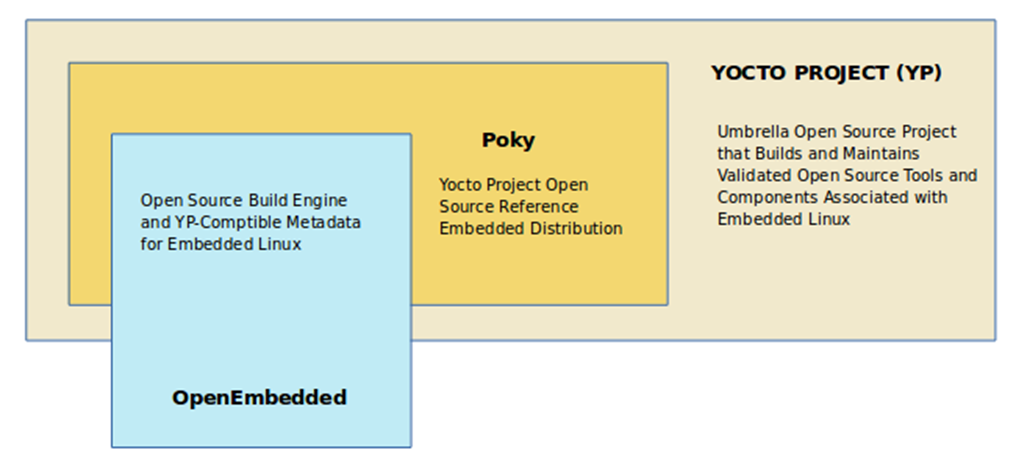
\includegraphics[width=1\linewidth]{Images/9_Linux_image/Poky and Yocto.png}
      \centering
    Hierarchical Architecture of Yocto Project 
    \label{fig:enter-label}
\\
\raggedright
\noindent \\
\textbf{Advantages}: Highly customizable, scalable, supports a wide array of hardware.\\
\textbf{Disadvantages}: Steeper learning curve, complex setup.\\


\subsection{Methodology}

\subsubsection{Buildroot Methodology}

 
    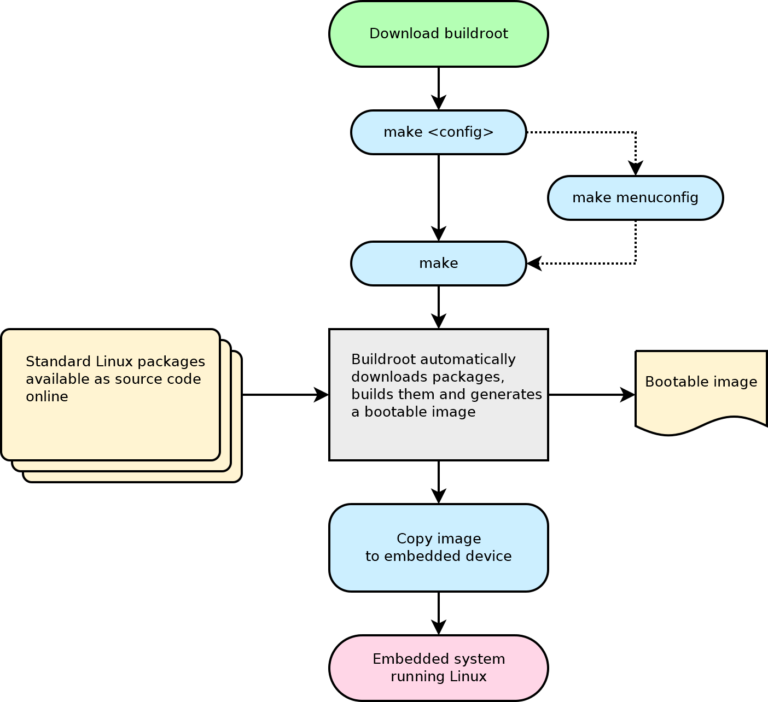
\includegraphics[width=1\linewidth]{Images/9_Linux_image/Buildroot Flowchart.png}
      \centering
    Buildroot Flowchart
    \label{fig:enter-label}
\noindent
\\
\raggedright
\paragraph{Overview}
This section outlines the steps taken to create a minimal Linux image for BeagleBone AI-64 and QEMU using Buildroot.

\paragraph{Materials and Tools}
\begin{itemize}
    \item \textbf{Hardware:} BeagleBone AI-64, development PC.
    \item \textbf{Software:} Buildroot, QEMU.
    \item \textbf{Tools:} Cross-compilation toolchain, terminal emulator, text editor.
\end{itemize}

\paragraph{Procedure}
\subparagraph{Initial Setup}
\begin{itemize}
    \item Download and install Buildroot from the official website: \\
     git clone https://gitlab.com/buildroot.org/buildroot.git
    \item Make sure that you update your current version of ubuntu \\
    sudo apt update \\
    sudo apt upgrade 
    \item You may not have installed ncurse already in your device use :\\
    sudo apt-get install libncurses5-dev libncursesw5-dev\\
    Note : ncurse is used for configuration of the image using make menuconfig which will be used later in this project.
      
\end{itemize}

\subparagraph{Buildroot Configuration}
\begin{itemize}
    \item Get into configs file to see what is there.\\
    ls configs/
    \item Select the appropriate target architecture (e.g., Aim for beagleboneai64\_defconfig or qemu\_x86\_64\_defconfig).
    \item Run `make menuconfig` in the Buildroot directory to open the configuration menu.
    \item Choose the necessary packages and kernel options for a minimal image.
    \item Save the configuration.\\
    Note : error may occur if ncurse library isn’t installed 
    
\end{itemize}
\noindent \\
        
        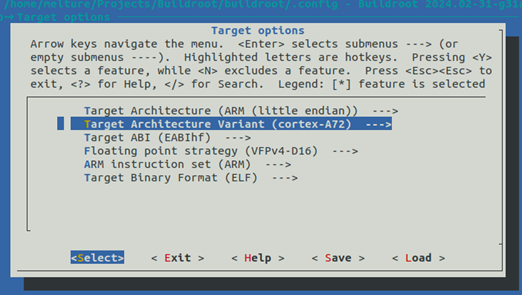
\includegraphics[width=1\linewidth]{Images/9_Linux_image/Buildroot Configuration Menu.png}
       \centering
        Configuration Menu
        \label{fig:enter-label}
        \\
    \raggedright
\subparagraph{Building the Image}
\begin{itemize}
    \item Execute `make` to start the build process.
    \item Monitor the build process for any errors or missing dependencies.
    \item Upon completion, locate the built image in the output directory.\\
    ls -la output/images/
    
\end{itemize}

\subparagraph{Testing the Image on QEMU}
\begin{itemize}
    \item Install QEMU on the development PC if not already installed.
    \item Run the built image on QEMU using the appropriate command. \\
    qemu-system-x86\textunderscore64 \
    -M pc \
    -kernel ./output/images/bzImage \
    -drive file=./output/images/rootfs.ext2,if=virtio,format=raw \
    -append ''root=/dev/vda console=ttyS0'' \
    -net user,hostfwd=tcp:127.0.0.1:3333-:22 \
    -net nic,model=virtio \
    -nographic

    \item Verify the boot process and basic functionality.\\
    try : echo , date ,...etc
\end{itemize}

\subparagraph{Testing the Image on BeagleBone AI-64}
\begin{itemize}
    \item Flash the built image onto an SD card using a tool like `dd` or Etcher. \\
    using dd :\\
    to upload image to SD-Card :\\
    First to list storage devices :\\
    lsblk\\
    Copy image bit by bit using sudo to have root privileges\\
    sudo dd if=”path of file to be copied” of=”destination to be copied to” bs=”set block size(1M)”\\
    Etcher will be displayed when using Yocto image later in this book

    \item Insert the SD card into the BeagleBone AI-64 and power it on.
    \item Verify the boot process and basic functionality on the actual hardware.\\
    verification can be done using picocom \\
    To get serial console from board we can install serial terminal \\
    sudo apt install -y picocom \\
    You may need to call out usermod in dialout group to avoid permission denied even using sudo \\
    sudo usermod -a -G dialout \$USER \\
    groups \$USER \\
    We can now use picocom  \\
    picocom -b “baud rate” “Path of device”  \\
    Reset the board and if you get login prompt then every thing works fine \\
    •	Type root and there is no password for login \\
    •	To write script use  \\
    vi “any name”.sh  \\
    type I to insert text \\
    after you finished press esc and type :wq \\
    •	Exiting picocom  \\
        \indent •	 Ctrl + A \\
        \indent •	 Ctrl + X \\

    
    
\end{itemize}

\paragraph{Troubleshooting and Optimization}
\begin{itemize}
    \item QEMU image run perfectly without graphic interface
    \item To optimize our images , only the necessary libraries are included while the rest are discarded however Any change repeat all this steps again (long time wasted)
\end{itemize}

\subsubsection{Yocto Methodology}

    
    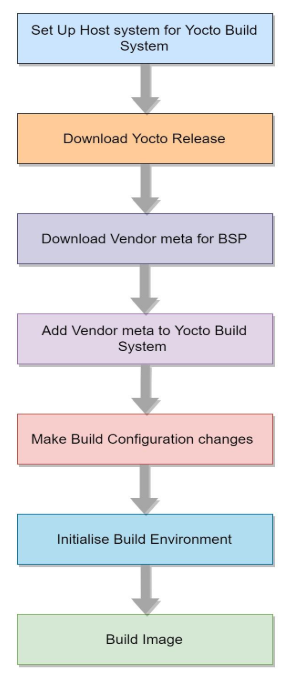
\includegraphics[width=0.4\linewidth]{Images/9_Linux_image/Yocto Flowchart.png}
    \centering \\
    Yocto Flowchart
    \label{fig:enter-label}
\\
\raggedright
\paragraph{Overview}
This section outlines the steps taken to create a minimal Linux image for BeagleBone AI-64 and QEMU using Yocto.

\paragraph{Materials and Tools}
\begin{itemize}
    \item \textbf{Hardware:} BeagleBone AI-64, development PC.
    \item \textbf{Software:} Yocto Project tools (BitBake, OpenEmbedded , poky distribution), QEMU.\\
    •	At least 90 Gbytes of free disk space, although much more will help to run multiple builds and increase performance by reusing build artifacts.\\
    \indent	 ~~~~* We use virtual machine of about 150 GB\\
    •	At least 4 Gbytes of RAM, though a modern modern build host with as much RAM and as many CPU cores as possible is strongly recommended to maximize build performance.\\
    \indent	We allocated 8 GB RAM for virtual machine \\
    •	Runs a supported Linux distribution (i.e. recent releases of Fedora, openSUSE, CentOS, Debian, or Ubuntu). For a list of Linux distributions that support the Yocto Project, see the Supported Linux Distributions section in the Yocto Project Reference Manual. For detailed information on preparing your build host, see the Preparing the Build Host section in the Yocto Project Development Tasks Manual. \\
    \indent ~~~~	• Git 1.8.3.1 or greater    \\
    \indent ~~~~	• tar 1.28 or greater       \\
    \indent ~~~~	• Python 3.8.0 or greater.  \\
    \indent ~~~~	• gcc 8.0 or greater.       \\
    \indent ~~~~	• GNU make 4.0 or greater   \\
    \indent ~~~~	• Python version 

    \item \textbf{Tools:} Cross-compilation toolchain, terminal emulator, text editor.
\end{itemize}

\paragraph{Procedure}
\subparagraph{Initial Setup}
\begin{itemize}
    \item Because the Yocto Project tools rely on the “python” command, you will likely need to alias “python” to “python3.” Edit your .bashrc file:\\
    vi \~ /.bashrc \\
    Scroll to the bottom and add the following to a new line (press ‘a’ to append new text):\\
    alias python=python3 \\
    Save and exit (‘esc’ followed by entering “:wq”). Re-run the .bashrc script to update your shell: \\
    source ~/.bashrc \\
    Check your Python version: \\
    python --version \\
    Note : It should say something like “Python 3.8.xxx.” \\
    
    \item Download and set up the Yocto Project environment from the official website:\url{https://www.yoctoproject.org/}.
    \item Install the required dependencies and tools for Yocto.\\
    \$ sudo apt install gawk wget git diffstat unzip texinfo gcc build-essential chrpath socat cpio python3 python3-pip python3-pexpect xz-utils debianutils iputils-ping python3-git python3-jinja2 libegl1-mesa libsdl1.2-dev python3-subunit mesa-common-dev zstd liblz4-tool file locales libacl1 \\
    \$ sudo locale-gen en\_US.UTF-8
    
    \item Clone the necessary Yocto layers, including `poky` \\
    git clone git://git.yoctoproject.org/poky.git \\
    cd poky \\
   
    
\end{itemize}

\subparagraph{Yocto Configuration}
\begin{itemize}
    \item Source the Yocto environment setup script: `source oe-init-build-env`.
    
    \item Configure the build environment by editing the `conf/local.conf` file.
    
    \item Specify the target machine in `conf/local.conf` (e.g., `MACHINE = "beaglebone-yocto"`) for BeagleBone AI-64.
    
    \item Add necessary layers using `bitbake-layers add-layer` command.\\
    \item      Add a Hardware Layer (arago) \\
    git clone git://git.yoctoproject.org/meta-arago \\
    bitbake-layers add-layer ../meta-arago \\


        
        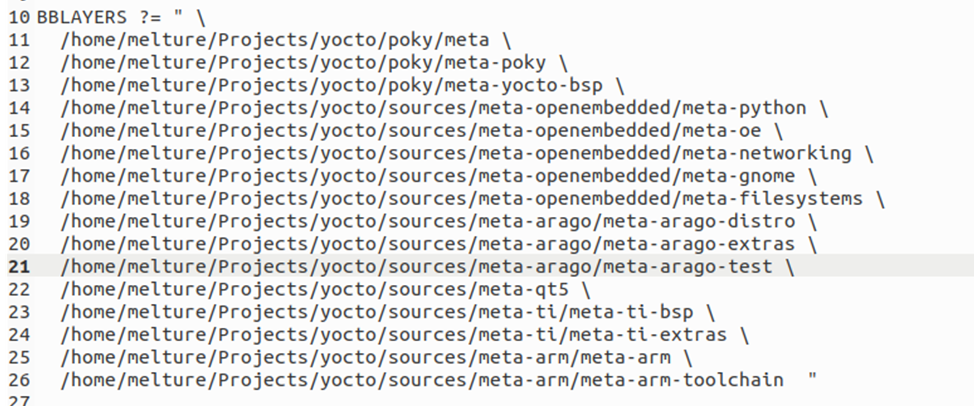
\includegraphics[width=1\linewidth]{Images/9_Linux_image/BBlayers.png}
\centering      
\\
Layers for Yocto Image
        \label{fig:enter-label}
\\


\end{itemize}
\raggedright
\subparagraph{Building the Image}
\begin{itemize}
    \item Execute `bitbake core-image-minimal` to start the build process.
    \item Monitor the build process for any errors or missing dependencies.
    \item Upon completion, locate the built image in the `tmp/deploy/images` directory.
\end{itemize}

\subparagraph{Testing the Image on QEMU}
\begin{itemize}
    \item Run the built image on QEMU using `runqemu` command.
    \item Verify the boot process and basic functionality.
   
       
        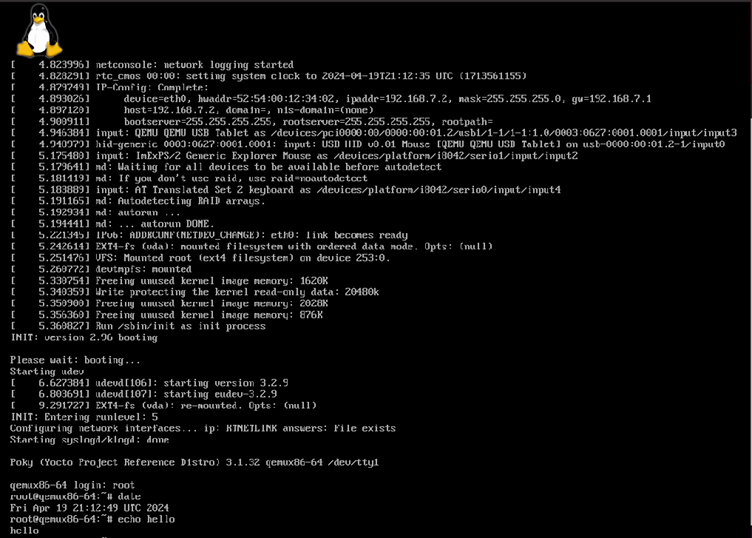
\includegraphics[width=1\linewidth]{Images/9_Linux_image/Yocto QEMU Image .png}
 \centering
\\
Yocto QEMU Image
        \label{fig:enter-label}

\end{itemize}
\raggedright
\paragraph{Testing the Image on BeagleBone AI-64}
\begin{itemize}
    \item Flash the built image onto an SD card using a tool like `dd` or Etcher.\\
    
       
        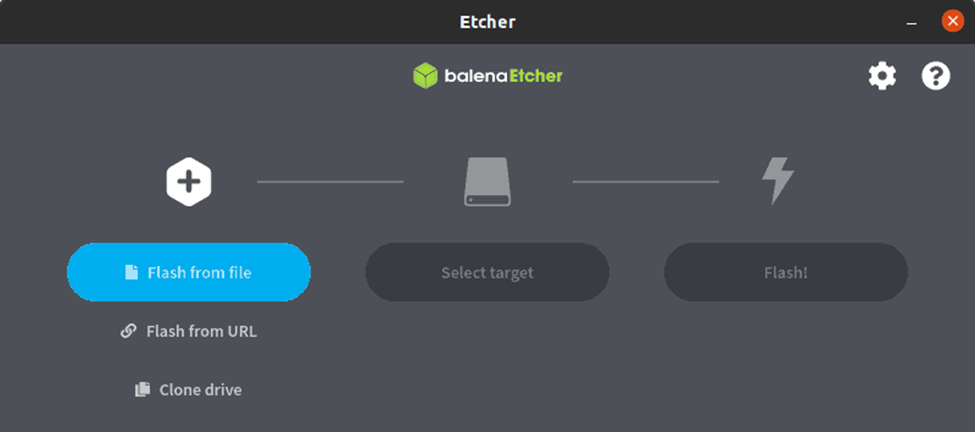
\includegraphics[width=1\linewidth]{Images/9_Linux_image/Etcher.png}
 \centering        
Etcher
        \label{fig:enter-label} 
\\
\raggedright 
    
    Note: if you are using Virtual Machine, you should mount SD Card or any disk connected to USB in main bar Input>USB and select disk you want to mount.
    \item Insert the SD card into the BeagleBone AI-64 and power it on. \\
    •	Then use picocom to monitor board behaviour : \\
        o	Connect FTDI cable to laptop and run the following commend to ensure it is read\\
        o	Change directory to /dev \\
        o	And look for ttyUSB0 \\
        o	Then prepare Picocom \\
        picocom -b 115200 /dev/ttyUSB0 \\
        o	Finally press boot button down and plug power supply don’t leave button until there is booting observed in the laptop \\
        o	Some tests can be made : \\
        uname -r \\
        uname -a \\
        lsblk \\

    \item Verify the boot process and basic functionality on the actual hardware.
\end{itemize}

\paragraph{Troubleshooting and Optimization}
\begin{itemize}
    \item Storage issue : due to large space needed by yocto project there was two options :\\
    1- use poky tiny : however poky tiny only reduces the size of image produced not the total storage consumed in the host and here is a brief comparsion between poky and poky tiny : \\
    \noindent
\centering
        \begin{tabular}{|| c c c ||}\hline
         term of Comparison  & Poky & Poky Tiny \\ 
         RootFS(MB) & 4 & 1 \\  
         Kernel(MB) & 7 & 2.7  \\  
         Boot time(Sec):  & 9.1 & 5.2 \\  
         Main Components & &  \\  
         Base-Utils & BusyBox & BusyBox \\  
         C Library & GLIBC & Musl \\  
         Dev manager & : Udev/Eudev & : busybox-mdev  \\
         Other & Util-linux  & busybox  \\
         \hline
        \end{tabular} 

\raggedright

    
   2 - Resolve storage issues by freeing up disk space as necessary.\\
   as mentioned early, building yocto image require minimum of 80 GB and it is recommended to have 150 GB to build multiple images.
   
    \item Handle any branch mismatch and BSP compatibility issues.\\
    More about the layers used in building Board Image: \\
1.	\textbf{meta}: This is the core layer of the Yocto Project, also known as Poky. It provides essential recipes, configurations, and tools for building Linux distributions using the Yocto build system. This layer includes basic system components and serves as the foundation for customizing Yocto-based distributions. \\
2.	\textbf{meta-poky}: This layer is part of the Poky reference system and provides configurations and recipes specific to the Poky distribution. It includes settings for the default system configuration, package management, and other Poky-specific features. \\
3.	\textbf{meta-yocto-bsp}: This layer contains Board Support Packages (BSPs) for various hardware platforms supported by the Yocto Project. It provides configurations and recipes tailored to specific boards, including kernel configurations, bootloader settings, and device tree files. \\
4.	\textbf{meta-arago/meta-arago-distro}: This layer is part of the meta-arago project, which focuses on supporting Texas Instruments (TI) platforms with the Yocto Project. The meta-arago-distro layer defines distributions specific to TI hardware, including configurations and recipes optimized for TI platforms like the BeagleBone series. \\ 
5.	\textbf{meta-arago/meta-arago-extras}: This layer provides additional components and configurations beyond the basic meta-arago-distro layer. It may include extra packages, optimizations, and features tailored for TI platforms. \\
6.	\textbf{meta-openembedded/meta-networking}: This layer, part of the OpenEmbedded project, provides recipes and configurations for networking-related software. It includes packages for network protocols, utilities, and services, enabling networking functionality in Yocto-based distributions. \\
7.	\textbf{meta-openembedded/meta-python}: This layer focuses on Python-related software and provides recipes for Python packages, libraries, and utilities. It includes tools for Python development, as well as Python bindings for various libraries and frameworks. \\
8.	\textbf{meta-openembedded/meta-oe}: This is a comprehensive layer within the OpenEmbedded ecosystem and contains a wide range of additional recipes and configurations beyond the core Poky layer. It includes packages for desktop environments, development tools, multimedia software, and much more. \\
9.	\textbf{meta-openembedded/meta-gnome}: This layer specializes in GNOME desktop environment-related packages and configurations. It includes recipes for GNOME desktop components, applications, and libraries, enabling the creation of Yocto-based distributions with GNOME desktop support. \\
10.	\textbf{meta-openembedded/meta-filesystems}: This layer focuses on filesystem-related software and provides recipes for various filesystem utilities, formats, and tools. It includes support for different filesystem types and features, such as encryption and compression. \\
11.	\textbf{meta-qt5}: This layer focuses on the Qt framework and provides recipes for Qt libraries, tools, and applications. It enables the development of graphical user interfaces (GUIs) using Qt on Yocto-based distributions. \\
12.	\textbf{meta-ti/meta-ti-bsp}: This layer is part of the meta-ti project, which focuses on supporting TI platforms with the Yocto Project. The meta-ti-bsp layer provides Board Support Packages (BSPs) for TI hardware, including configurations and recipes tailored to specific TI platforms. \\
13.	\textbf{meta-ti/meta-ti-extras}: Similar to meta-arago/meta-arago-extras, this layer provides additional components and configurations specific to TI platforms. It may include extra packages, optimizations, and features beyond the basic meta-ti-bsp layer. \\
14.	\textbf{meta-arm/meta-arm}: This layer provides additional support for ARM-based architectures within the Yocto Project. It includes configurations, recipes, and optimizations for building distributions targeting ARM-based hardware platforms. \\
15.	\textbf{meta-arm/meta-arm-toolchain}: This layer focuses on toolchain support for ARM architectures. It provides recipes and configurations for cross-compilation toolchains targeting ARM-based systems, enabling development and deployment of software on ARM platforms. \\
16.	\textbf{meta-virtualization}: This layer provides support for virtualization-related software and technologies within the Yocto Project. It includes recipes for virtualization tools, hypervisors, and related components, enabling the creation of Yocto-based distributions for virtualized environments. \\

image were built based on Krikstone branch and the reason for choosing this branch specifically was : \\
Choosing criteria:
the yocto release must line up with poky reference distribution
the yocto release must have long term support (upto 2 years)
the codename need to line up with yocto version (check second column)
latest stable release and/or Long Term Support : \\


\centering 
 Yocto Releases Comparison \\

\label{tab:my_label}
\raggedright
\noindent
    \begin{tabular}{|c|c|c|c|c|} \hline 
 Codename& Yocto Version& Release Date& Current Version&Support Level\\ \hline 
         Kirkstone (like 'kirk stun')&  4.0&  May 2022&  4.0.16 & until Apr. 2026\\ \hline 
         Dunfell&  3.1&  April 2020&  3.1.31 & until Apr. 2024\\ \hline
    \end{tabular}
    
    
\raggedright

In addition to selecting the release based on queries and Beagle Bone Community : \url {https://forum.beagleboard.org/t/bbai-64-yocto-bsp-support/32813/6 } \\
so each layer must be converted to the same layer so that this error is resolved.


    \item Address `do\_fetch` task failures by ensuring local access to required resources.\\
       
        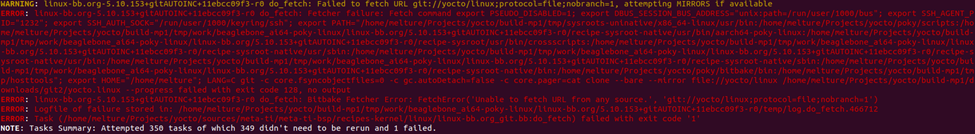
\includegraphics[width=1\linewidth]{Images/9_Linux_image/Do Fetch Problem log.png}
 \centering       
do\_fetch error log
        \label{fig:enter-label}
  \\
\raggedright
    \indent 
    ~to solve it you must make sure that git is configured to allow access to \indent ~local files using the following command :\\
    \indent ~ \indent ~git config --global core.longpaths true  \\
    \indent ~and check that this command was done using : \\
   \indent ~\indent~git config --list \\
    Note: Usually "do\_fetch"  stuck error is caused by network issue. \\ Please check your network or change a new network and try in different time. \\
    If you have used yocto to compile successfully before, you can directly copy the relevant files downloaded before to the current project. This way you can skip the "do\_fetch" step. \\

   

\end{itemize}

\subsection{Results}
the produced image will have name of core-image-minimal-beaglebone-ai64.wic.xz
xz is compressed version of image.

\subsubsection{Buildroot Image Results}
The process of building the Linux image using Buildroot was completed successfully for the QEMU . The image was built without significant issues, and the following results were obtained:
\begin{itemize}
    \item \textbf{QEMU:} The Buildroot image booted successfully in the QEMU emulator, demonstrating basic functionality.
\end{itemize}

\subsubsection{Yocto Image Results}
Building the Linux image using Yocto presented several challenges, including disk space limitations and branch mismatches. However, these issues were resolved, and the following results were obtained:
\begin{itemize}
    \item \textbf{QEMU:} The Yocto image booted successfully in the QEMU emulator after addressing initial configuration issues.
    \item \textbf{BeagleBone AI-64:} The Yocto image was built and flashed onto the BeagleBone AI-64. Despite initial do\_fetch task failures, the final image booted successfully after resolving local access requirements.
\end{itemize}

\subsubsection{Comparison of Buildroot and Yocto Images}
\begin{itemize}
    \item \textbf{Build Time:} Buildroot images were quicker to build compared to Yocto images, which required more configuration and build time.
    \item \textbf{Customization:} Yocto provided more customization options and granular control over the build process.
    \item \textbf{Performance:} Both images performed comparably in basic tests on QEMU and BeagleBone AI-64, but further testing is required for a detailed performance comparison. 
\end{itemize}

beaglebone.org also provide a pre-built image by looking to the size of pre-built image is about 537 MB while our built image is about 36 MB so the used storage size will reduce to about \textcolor{red}{6.7\%} making the proposed image more optimized than the one provided by beaglebone.org
%\subsection{Performance Metrics}
%\begin{tabular}{|c|c|c|}
%\hline
%\textbf{Metric} & \textbf{Buildroot (QEMU)} & \textbf{Yocto (QEMU)} \\
%\hline
%Boot Time (s) & 15 & 18 \\
%Memory Usage (MB) & 40 & 45 \\
%Disk Usage (MB) & 60 & 65 \\
%\hline
%\end{tabular}

%\begin{tabular}{|c|c|c|}
%\hline
%\textbf{Metric} & \textbf{Buildroot (BeagleBone AI-64)} & \textbf{Yocto %(BeagleBone AI-64)} \\
%\hline
%Boot Time (s) & 20 & 22 \\
%Memory Usage (MB) & 50 & 55 \\
%Disk Usage (MB) & 70 & 75 \\
%\hline
%\end{tabular}

\subsection{Discussion}

\subsubsection{Analysis of Build Processes}
The build processes for both Buildroot and Yocto demonstrated unique advantages and challenges. Buildroot was straightforward and efficient, making it suitable for quick and simple builds. Yocto, while more complex, offered greater customization and control, which is beneficial for more advanced and specific requirements.

\subsubsection{Performance Interpretation}
The performance metrics indicated that both Buildroot and Yocto images performed similarly in basic tests. However, Yocto's additional customization options could lead to better optimization in more complex scenarios. The slightly higher resource usage in Yocto images is a trade-off for its flexibility.

\subsubsection{Advantages and Disadvantages}
\begin{itemize}
    \item \textbf{Buildroot:} The main advantage of Buildroot is its simplicity and speed. It is ideal for projects that require a minimal and quick setup. The disadvantage is its limited customization compared to Yocto.
    \item \textbf{Yocto:} Yocto offers extensive customization and is well-suited for complex and specific project requirements. The downside is its complexity and longer build times.
\end{itemize}

\subsubsection{Challenges and Solutions}
Several challenges were encountered during the build process, particularly with Yocto. Disk space limitations were a significant hurdle, requiring careful management of resources. Branch mismatches and do\_fetch task failures were resolved through diligent troubleshooting and configuration adjustments.

\subsubsection{Recommendations for Future Work}
Future work should focus on further optimization of the Yocto build process to reduce build times , include project required packages and resource usage. Additionally, comprehensive performance testing should be conducted to fully evaluate the performance of Yocto images in various scenarios.

\subsection{Conclusion}

This project successfully demonstrated the process of building minimal Linux images for the BeagleBone AI-64 and QEMU using both Buildroot and Yocto. The results highlighted the trade-offs between the simplicity and efficiency of Buildroot and the customization and flexibility of Yocto.

Key findings include:
\begin{itemize}
    \item Buildroot is ideal for quick, simple builds with minimal configuration.
    \item Yocto offers extensive customization, making it suitable for more complex and specific requirements.
    \item Both methods produced functional images, with comparable basic performance metrics.
\end{itemize}

The project faced several challenges, particularly with the Yocto build process, which were successfully addressed through troubleshooting and configuration adjustments. The successful creation of functional images for both QEMU and BeagleBone AI-64 demonstrates the project's success and provides a foundation for further work.

Future work should focus on optimizing the Yocto build process, conducting comprehensive performance testing, and exploring additional features and customizations. This project contributes valuable insights into the process of building Linux images for embedded systems, with implications for both academic research and practical applications. \\

\iffalse
\subsection{References}
- Dealing with txt file in terminal command window : \\ \url{https://www.makeuseof.com/vim-vi-delete-line/#:~:text=Highlight%20the%20line%20you%20want,several%20lines%20one%20by%20one}. \\
- Overview Manual : \url{https://docs.yoctoproject.org/2.5/overview-manual/overview-manual.html#openembedded-build-system-workflow }\\
- Tutorial : \url{https://www.youtube.com/watch?v=zNLYanJAQ3s} 
- Yocto image for BBB : \url{https://www.youtube.com/playlist?list=PLzJTJ1FSIHJtn5gj6oLWnrDpd6dXPSbbG }\\
- Yocto Tutorial : \url{https://www.digikey.com/en/maker/projects/intro-to-embedded-linux-part-2-yocto-project/2c08a1ad09d74f20b9844e566d332da4}\\
- Yocto Customize : \url{https://youtube.com/playlist?list=PLdUUBf0zT0W9ihkrxXMqK7jf2_wt2xzFS&si=uUR5m9Vlxr9pEu_f }\\
\url{https://youtu.be/6yziQuLvyIE?si=PUi6fnPXijjz6SM2 }\\
- Splash Screen : \url{https://easylinuxji.blogspot.com/2019/03/replace-default-splash-screen-in-yocto.html}\\
- Virtual Machine initial Problems solutions: \url{https://www.youtube.com/watch?v=w4E1iqsn_wA }\\
-  Book Link : \url{https://www.pdfdrive.com/linux-programming-by-example-e165312568.html} \\
- Yocoto Project :  \url{https://www.yoctoproject.org/}\\
- Embedded Linuxs : \url{https://www.youtube.com/playlist?list=PLEBQazB0HUyTpoJoZecRK6PpDG31Y7RPB }\\
- Linuxs Kernel : \url{https://youtu.be/QatE61Ynwrw?si=O3NCac2n1jQIir3O }\\
- Buildroot and Yocto Tutorial : \url{https://mkaczanowski.com/embedded-development-with-qemu-beagleboard-yocto-angstrom-buildroot-where-to-begin/ }\\
- Embedded Vision : \url{https://www.edge-ai-vision.com/2019/10/building-complete-embedded-vision-systems-on-linux-from-camera-to-display-a-presentation-from-montgomery-one/ }\\
- all about bash script :\url{https://www.freecodecamp.org/news/bash-scripting-tutorial-linux-shell-script-and-command-line-for-beginners/#:~:text=A%20bash%20script%20is%20a,process%20using%20the%20command%20line} \\
- Automated Testing using Script : \url{https://www.youtube.com/watch?v=CvLm5Ftv6XI }\\
\fi


\newpage
\section{Conclusion}
\newpage
\section{Future work}

\newpage
\printbibliography
\newpage
\section*{Appendix}


%____________________ To Be Removed _______________________
\newpage
\section{section}

% for numbered list
\begin{enumerate}
    \item if want multiple items
\end{enumerate}
%----------------------------

% for bullet points
\begin{itemize}
    \item if want multiple items
\end{itemize}
%----------------------------

% for math equ
\begin{equation}
    \centering
    for\_equation = write here 
    \label{0}
\end{equation}
%----------------------------

\subsection{Source Code} 

%----------------------------
% for citation
as mentioned in this reference \cite{ref} %put the lable of the reference inside
%----------------------------

%----- adding code-----------
\subsubsection{code section title}
\lstinputlisting[language=Python, caption=Python Code Example]{Codes/C.py}
%----------------------------

%----adding image------------
%1. single image

 \begin{figure}[!h]
     \centering
     
\includegraphics[scale =0.3]{Images/ALEXU_1.jpg}
     \caption{image caption}
     \label{fig:enter}
 \end{figure}

%2. two images
\begin{figure}[!h]
  \centering
  \begin{minipage}[b]{0.47\textwidth}
    
\includegraphics[width=\textwidth]{Images/ALEXU_1.jpg}
    \caption{adding 2 images }
  \end{minipage}
  \hfill
  \begin{minipage}[b]{0.47\textwidth}
    
\includegraphics[width=\textwidth]{Images/ALEXU_1.jpg}
    \caption{adding 2 images}
  \end{minipage}
\end{figure}
%----------------------------

%---- adding tables -----------
\begin{table}[h!]
\begin{center}
\begin{tabular}{||c c c c||} 
 \hline
 Col1 & Col2 & Col2 & Col3 \\ [0.5ex] 
 \hline\hline
 1 & 6 & 87837 & 787 \\ 
 \hline
 2 & 7 & 78 & 5415 \\
 \hline
 3 & 545 & 778 & 7507 \\
 \hline
 4 & 545 & 18744 & 7560 \\
 \hline
 5 & 88 & 788 & 6344 \\ [1ex] 
 \hline
\end{tabular}
\end{center}
\caption{Table to test captions and labels.}
\label{table:1}
\end{table}
%----------------------------
\begin{table}[h!]
\begin{center}
\begin{tabular}{|c|}


\includegraphics[width=\textwidth]{Images/ALEXU_1.jpg}

\end{tabular}
\end{center}
\caption{aloooooooooooo}
\label{table:1}
\end{table}

\end{document}
